\chapter{Eksperymenty}

\section{Pierwszy krok kaskady - lokalizacja frontu autobusu}

\subsection{Zbiór danych uczących i testowych}

Pierwszą partią danych ucząco-testowych było 11 zestawów obrazów
przygotowanych z~uprzednio pobranych filmów z~serwisu YouTube.

Każdy zestaw składał się z co najmniej dwuch zbiorów obrazów 
reprezentujących oznaczone fronty autobusów oraz obrazy tła
(ang. background). Opcjonalnym zbiorem był zestaw oznaczonych 
frontów autobusów typu solaris. Osobny zestaw frontów miał na celu
porównanie skuteczności detektorów przygotowanych tylko przy pomocy
pojedynczego typu obiektu oraz tych do przygotowania których użyto
obiektów znacząco od siebie różnych.

\subsubsection{Zbiór jJ9ixBfVR5k}

\begin{figure}[!h]
    \centering
    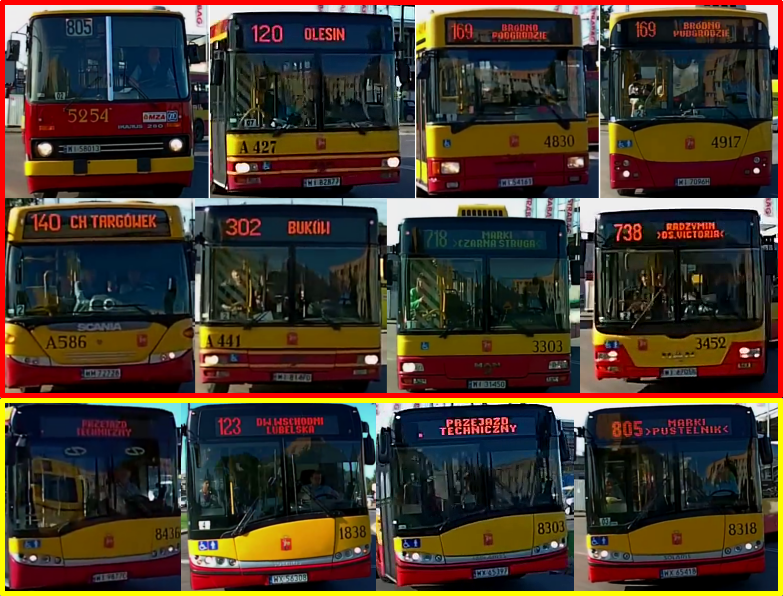
\includegraphics[width=0.9\textwidth]{img/exp_trainig_data_jJ9}
    \caption{Typy autobusów zawarte w zbiorze jJ9ixBfVR5k}
    \label{fig:jJ9ixBfVR5k_types}
\end{figure}

\begin{table}[!h]
    \centering
    \begin{tabular}{c|c|c}
        Front   & Solaris   & Background \\
        2587    & 222       & 2239
    \end{tabular}
    \caption{Liczebność zbioru jJ9ixBfVR5k}
    \label{tab:jJ9ixBfVR5k_count}
\end{table}

\subsubsection{Zbiór vYqZ4-tH4M0}

\begin{figure}[!h]
    \centering
    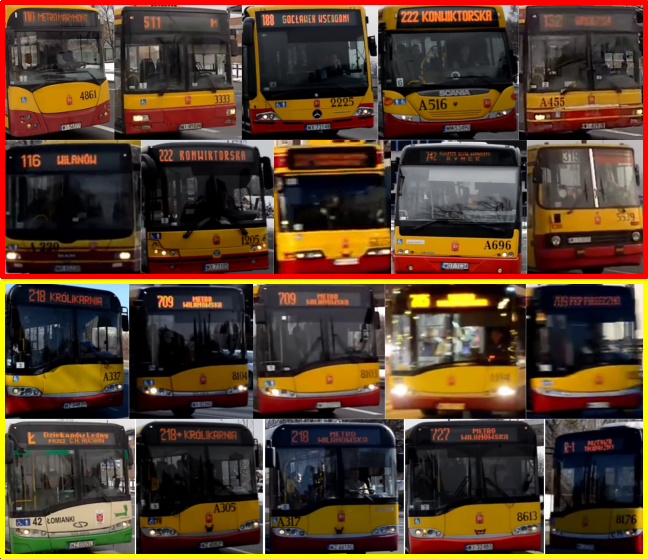
\includegraphics[width=0.9\textwidth]{img/exp_trainig_data_vYq}
    \caption{Typy autobusów zawarte w zbiorze vYqZ4-tH4M0}
    \label{fig:vYqZ4-tH4M0_types}
\end{figure}

\begin{table}[!h]
    \centering
    \begin{tabular}{c|c|c}
        Front   & Solaris   & Background \\
        2587    & 222       & 2239
    \end{tabular}
    \caption{Liczebność zbioru vYqZ4-tH4M0}
    \label{tab:vYqZ4-tH4M0_count}
\end{table}

Pierwsza iteracja uczenia detektorów miała na celu przetestowanie
opcji jakie można zadać narzędziu uczącemu - opencv\_traincascade.

Za zbiór testowy posłużył zestaw oznaczonych zdjęć oraz zdjęć tła
przygotowany dla filmu o id jJ9ixBfVR5k:
\begin{itemize}
\item oznaczone fronty: 2587,
\item oznaczone fronty typu solaris: 222,
\item obrazy tła: 2239.
\end{itemize}

Pierwszy test miał za zadanie wyłonić najefektywniejszą metodę, do dalszych
eksperymentów. Narzędzie dostarczone wraz z~pakietem OpenCV - wspomniany
już opencv\_traincascade - umożliwia ,,wyszkolenie'' trzech rodzai
detektorów:

\begin{itemize}
    \item detektor wykorzystujący tzw. cechy Harra - wartość 
        domyślna (HAAR),
    \item detektor LBP,
    \item detektor HOG.
\end{itemize}

\begin{table}[!h]
    \centering
    \begin{tabular}{r|c|c|c|l}
        & HAAR         & LBP        & HOG              &       \\
        \hline
Solaris & 151  (43\%)  & 81  (23\%) & 61 (17\%)        & /346  \\
Różne   & 1051 (35\%)  & 748 (25\%) & 712 (24\%)       & /2925 \\
Tło     & 635  (11\%)  & 386 (6\%)  & 447 (7\%)        & /5588 \\
    \end{tabular}
    \caption{Porównanie skuteczności detektorów typu HAAR, LBP i HOG.}
    \label{tab:haar_lbp_hog_comparison}
\end{table}

Czas uczenia poszczególnych detektorów różnił się dość znacząco. Proces
uczenia detektora Haar-a trwał ponad 6 godzin, podczas gdy dla detektorów
BLP oraz HOG były to odpowiednio 42 minuty oraz 3 godziny i 10 minut.

